\section{Electronics} \label{sec:elec}

\subsection{Requirements}

% ===== Relation to System Level Requirements ===== %
The requirements for the electronics subsystem are listed below.
\begin{itemize}
\item The subsystem should be rechargeable and the charging time should be less than 5 hours. % olm bu dogru mu su an 13 saat falan demisiz asagida :D 

\item Rechargeable batteries should be non-removable.
\item Battery duration should be at least 5 hours.
\item The subsystem should be wired correctly and properly.
\item The subsystem should be able to operate during charging.
\item The subsystem should be able to operate Raspberry Pi.
\item The subsystem should be able to drive the servo motor.
\item Power consumption of the subsystem should be minimum. % not measurable
\item Status of the food supply should be observable.
\item Battery level for both charging and operation modes should be observable.
\item The subsystem should be able to measure the weight of a cat.
\item The subsystem should be able to deter dogs from the area without causing any harm.
\end{itemize}

\subsection{Solution}

% ===== Power consumption ===== %


 
 
 
 \subsubsection{Computer}
 
 The system runs on a computer. Raspberry pi zero wh is selected as the computer since it provides the required operations, which are listed below. 
 
\begin{itemize}
\item Getting images from the camera module.
\item Connecting to the server for fast classification.
\item Controlling the rotation of the motor by generating PWM signals.
\item Measuring the distance coming from the ultrasonic sonar sensor.
\item Measuring the weight of the animal coming from load sensor.
\item Receiving the analog battery voltages to indicate battery level in the web interface.
\item Controlling the LEDs which indicate detection of cats/dogs.
\item Controlling the LEDs which indicate the battery level.
\item Controlling the dog deterring system.
\end{itemize}
 
 
 Getting the images from the camera and connecting with the server are explained in the 'Integration of the Subsystems' section. All other operations will be explained in detail in the following modules.
 
  \subsubsection{Camera}
  
  A high quality camera is required in order to obtain successful classification results. Two different cameras can be used.
 
 \paragraph{Part A} Raspberry Pi Camera Module
 
 Raspberry pi has an input socket for its camera module. The camera is run by the GPU without CPU assistance. A 5 Megapixels sensor is used in this camera. A 15-pin Camera serial interface (CSI) is used to attach the camera to the device, and this interface is capable of high data transmission rates. Hence, the communication with the device to extract frame data is fast. With this camera, high-quality images can be obtained in a very small time interval. This camera, with dimensions of 20x25x9mm, will be placed in an apparatus for protection.
 

 Properties of the camera module are listed below \cite{cite:picammod}:
 
\begin{itemize}
\item Horizontal field of view 53.50 degrees.
\item Vertical field of view 41.41 degrees.
\item Focal length 3.60mm.
\end{itemize}
 
 
 \paragraph{Part B} Webcam
 A webcam can be connected to the USB input of the Raspberry Pi. Raspberry Pi USB input is run by CPU. Since there will be different operations on the CPU, the extraction of frame data will be slower. Also, even if \% 100 of the CPU is used for frame data transmission, the frame rate is still much lower than using the camera on the GPU. In order to obtain faster results, the image resolution should be decreased. However, if the image quality decreases significantly, classification operation might not work as accurately.
 

  \subsubsection{Motor}
  
    In the mechanics part, the gate mechanism is explained in detail. Two different positions of the gate are required. These two positions can be adjusted by two different ways.
 
 \paragraph{Part A} Servo Motor
  
  The positions can be adjusted by changing the duty cycle of the PWM signal of the servo motor.
  
  There are 3 connection wires to the servo motor. The power and ground inputs are connected to the outputs of separate voltage regulators, and the control wire is connected to the PWM GPIO port of the raspberry pi.
  
  A PWM signal is generated with a python script implemented in the raspberry pi. Maximum and minimum positions of the motor are selected as the operating positions. When the gate is to be opened, duty cycle is switched to \%2.5, and when the gate is to be closed, duty cycle is switched to \%12.5.
  
  The motor can operate between 4.8 and 7.2 Volts. The selected operation voltage is 6.6V which is close to the maximum voltage, but a safety margin is set. The output torque of the motor is around 12 kgF-cm, which is more than enough to rotate the gate under full load. \cite{cite:servomotor}
  
 
 \paragraph{Part B} DC Motor
 
 A DC Motor can be used to rotate the gate. A DC motor is a two wire continuous rotation motor, where the wires are power and ground wires. DC motor is also controlled by PWM signals. However, the power wire is controlled by turning it on and off. The motor should be on until it reaches to the required position and then turned off. This opening and closing operation might not be precise since the motor rotates very fast.
 
Also, more power will be dissipated in the DC motor than the servo motor. 
 
 
 
 
 
   \subsubsection{Measuring the Food Level}
   
   The users will be informed about the remaining food level in the reservoir. The food level can be measured by two different methods indicated below.
 
 \paragraph{Part A} Ultrasonic Sonar Sensor 
 
 An HC-SR04 ultrasonic sonar distance sensor can be used to measure the distance between the food and sensor. The sensor generates an ultrasonic sound around 40kHz. However, the amplitude of this sound is very low in order not to disturb the animals. The sensor contains two different transducers. The first transducer generates the sound wave, and the second transducer receives the echo of the transmitted wave. The distance is calculated by the following formula:
 
\begin{equation}
\text{distance = time $\times$ speed of sound  /  2}
\end{equation} % ;) :*

The generated sound is transmitted from the transducer, then the wave bounces back from the object; the returned wave is received from the second transducer. The distance is divided by 2 since the sound makes a round trip between the sensor and the food.

Sound speed is taken as 340 meters per second. 

The sensor has 4 pins: VCC, GND, ECHO, and TRIGGER \cite{cite:sonar}.
VCC pin is connected to one of the power outputs of the raspberry pi, and ground is connected to the common ground. Trigger pin is the digital output pin of the sensor; it can be considered as the transmitter transducer, and it is connected to the PWM output pin of the raspberry pi. Echo pin is the digital input pin of the sensor. A trigger signal is applied and the time is measured until the echo pin returns high value.

 
 \paragraph{Part B} Infrared Distance Sensor
 
 An infrared distance sensor such as GP2Y0A710K0F can be used in order to measure distance. The infrared sensor returns more accurate results than the ultrasonic sonar sensor. However, it is much more expensive than the ultrasonic sonar sensor.
 
 The operation principle is similar to the ultrasonic sonar sensor. An IR distance sensor uses a beam of infrared light and the reflected light from the object is received in the light detector position sensing part. When the position of the object changes, the angle of the reflected beam changes, and the distance is calculated from the angle change. A built-in signal processing circuit is included in the sensor to measure distance. The sensor returns analog voltage values as output with respect to the distance between sensor and object. \cite{cite:infrared}
 
    \subsubsection{Measuring the Weight}
  
A weight sensor is used in order to obtain additional information about the cats.

%% last sentence was red, may need to be checked
%% =========== FATIH - TODO =========== %%

% fatih weight sensorunu ne icin kullancaz biliyorsan yazar mısın

%% =========== FATIH - TODO =========== %%



  
  The sensor has three input wires. Power will be supplied from the raspberry pi, and ground will be connected to the common ground. The output wire returns analog voltage values with respect to the applied force on sensor. The analog voltage should be converted into digital data. An analog to digital converter HX711 integrated circuit will be used, and the digital data will be read though a port in the raspberry pi and scaled according to the measured weights.\cite{cite:hx711}
    
    \subsubsection{Battery}

The battery is one of the most important components of the project, since the system will not operate without a power supply. Two different power supply units will be used to supply raspberry pi and motor units separately in order to decrease motor noise.

In order to satisfy battery requirements, three different solution plans are considered.

\paragraph{Part A}
 18650 Lithium-Ion Batteries are selected as power supply since they are rechargeable and portable. Capacity of the battery will be determined from the current values when all subsystems are integrated. Increasing the capacity can be done with shunt connected batteries.
 
\paragraph{Part B}
 As an alternative, lithium-polymer batteries can be used. They are also rechargeable and portable. Furthermore, their capacity is higher compared to Li-Ion batteries. However, Li-Ion batteries are both cheaper and safer.
 
 \paragraph{Part C} 
 A power bank can be used. The capacity of a power bank is higher than the other 2 solutions, but the cost is also higher. This solution might be the most stable power supply. However, it is not cost efficient.
 
 
 
 2600 mAh 18650 Li-Ion batteries are selected after the current measurements. 2 batteries are shunt connected for the raspberry pi unit and 2 batteries are shunt connected for the servo motor unit. By this way, 5200 mAh capacity is obtained for each unit. These values are calculated with respect to the maximum drawn currents. However, the required operations consume much less current than these values. Hence, the overall system is able to operate at least 5 hours on this battery setup.
 
 
 \subsubsection{Battery Charger}
 
 The charging operation is done by using TP4056 1A lithium battery charger circuits. Since two different power supplies are used, two different charger circuits are connected. One of the charger circuits is connected to an electric socket from its micro-USB input. Input of the other charger circuit is connected in parallel to the first charger circuit. By this connection, when adapter is connected to the box, both charger modules will operate. Outputs of the charger circuits are connected to the inputs of shunt connected batteries. By this way, while the batteries are being charged, other subsystems can operate.
 
 For Li-Po batteries, same charging mechanism can be used.
 
 If power bank is used, there will be no charging mechanism. The micro-USB adapter will be directly connected to the power bank.
 
 
 \subsubsection{Voltage Regulators}
 
 Stable voltage is required to operate the raspberry pi and the motor.
 The raspberry pi requires a 5V 1.2A power supply. 1.2A is the maximum stall current. This requirement is satisfied by using a 5V 1.2A DC to DC boost voltage regulator. Two parallel connected batteries give 3.7V and the total capacity is 5200 mAh. The shunt connected battery is directly connected to a 5V 1A regulator. The output of the regulator is not ideal, but nonidealities do not affect the operation of the raspberry pi.
 The USB port of the regulator is used and the raspberry pi is powered from its micro-USB input.
 
The selected operation voltage of the servo motor is 6.6V. An XL6009 adjustable DC to DC boost converter is used. The regulator can supply output current up to 4A and the stall current of the servo motor is 2.5A. Hence, both voltage and current requirements are satisfied. However, cooling of this regulator is insufficient. It might be switched with a better regulator.

Input voltages for both regulators are between the range of Li-Ion Battery voltages. The overall system can operate when the batteries are empty and charging, as well as when they are full.

  \subsubsection{Dog Deterring}
  
Dog deterring module is explained in the 'Mechanics' section of this report.

\subsection{Risks}

% ===== Indicate alternative solutions ===== %
Possible risks for the electronics subsection are listed below.

\begin{itemize}
\item Voltage difference between shunt connected batteries.
\item Low output torque from servo motor.
\item Unstable PWM signal generation. 
\item Unstable voltage regulator outputs.
\item Wiring faults.
\item Grounding faults.
\end{itemize}


\subsection{Tests}


  \subsubsection{Tests Procedure}
  
  %Test Procedure is explained below.
\begin{itemize}
\item Measure the voltage of batteries.
\item Charge the batteries with charger circuits until the voltages are balanced.
\item Connect batteries to regulators.
\item Measure the output voltage of regulators for different voltages inside the voltage range of battery.
\item Power up the raspberry pi and the motor.
\item Connect the GPIO pins, camera, sonar sensor.
\item Measure the distance with sonar sensor.
\item Drive the motor.
\item Obtain images from the camera.
\item Measure the maximum and minimum camera view distance.
\item Drive the motor while camera is active.
\item Measure the distance while motor and camera are active.
\end{itemize}
% ===== Procedure and results of tests ===== %
  \subsubsection{Tests Results} 
\begin{itemize}
\item Li-Ion batteries operates properly. Output voltage is between 3.7V and 4.2V.
\item Parallel charging for two different power supply units operates correctly.
\item Batteries work while charging.
\item 5V 1.2A regulators return 5.35Volts when the  input is 3.7V  and 5.45 Volts when the input is 4.2V.
\item Adjustable regulator operates correctly, however its cooling system is not sufficient.
\item Measured distances can be seen in Figure~\ref{fig:sonardist}.


\begin{figure}[ht]
     \centering
     \begin{subfigure}[b]{0.49\textwidth}
     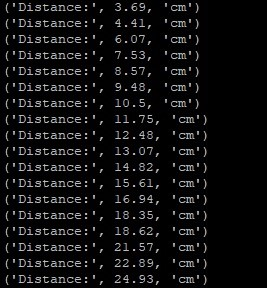
\includegraphics[width=\linewidth]{img/sonardistance-1.jpg}
     \label{fig:sonar1}
     \end{subfigure}
     \begin{subfigure}[b]{0.49\textwidth}
     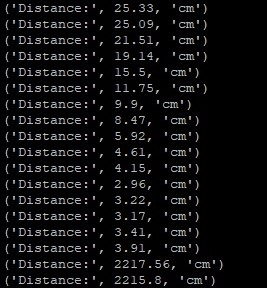
\includegraphics[width=\linewidth]{img/sonardistance-2.jpg}
     \label{fig:sonar2}
     \end{subfigure}        
     \caption{Measured Distances From Ultrasonic Sonar Sensor}
     \label{fig:sonardist}
\end{figure}


\item Motor is rotated according to the entered duty cycle values. For \%2.5 and \%12.5 duty cycles which are the on and off positions for the mechanical gate, generated PWM signals can be seen in Figure~\ref{fig:pwmaaa}.
\begin{figure}[ht]
     \centering
     \begin{subfigure}[b]{0.49\textwidth}
     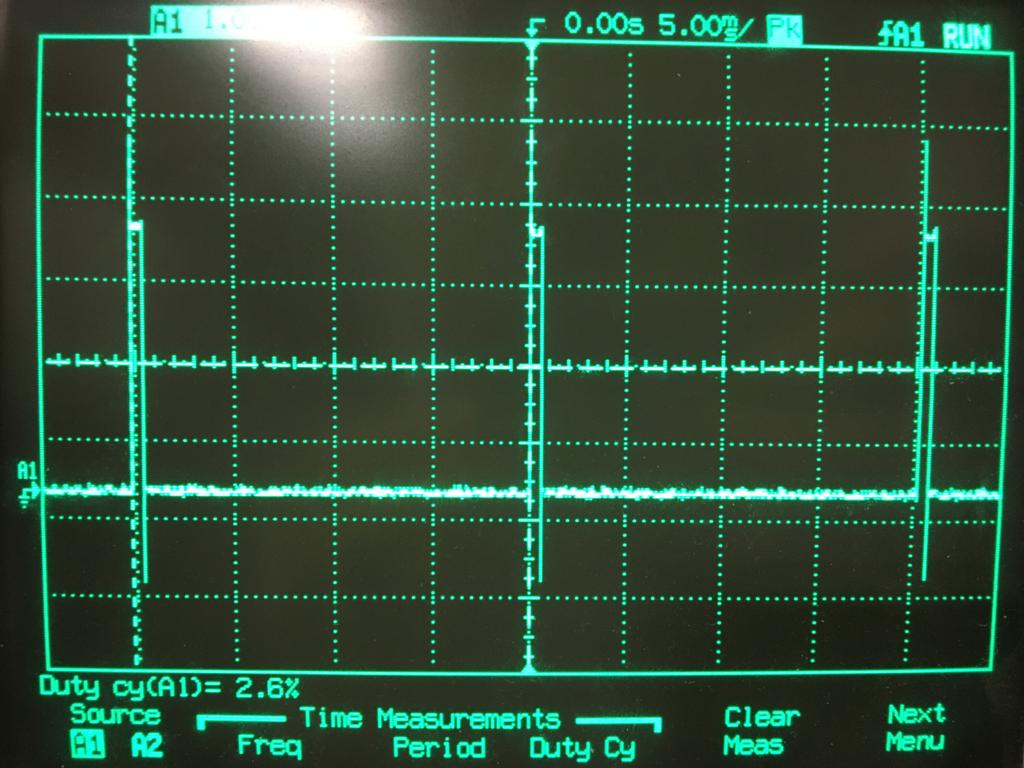
\includegraphics[width=\linewidth]{img/pwm25.jpeg}
     \caption{PWM Signal Duty Cycle = 2.5}
     \label{fig:pwm25}
     \end{subfigure}
     \begin{subfigure}[b]{0.49\textwidth}
     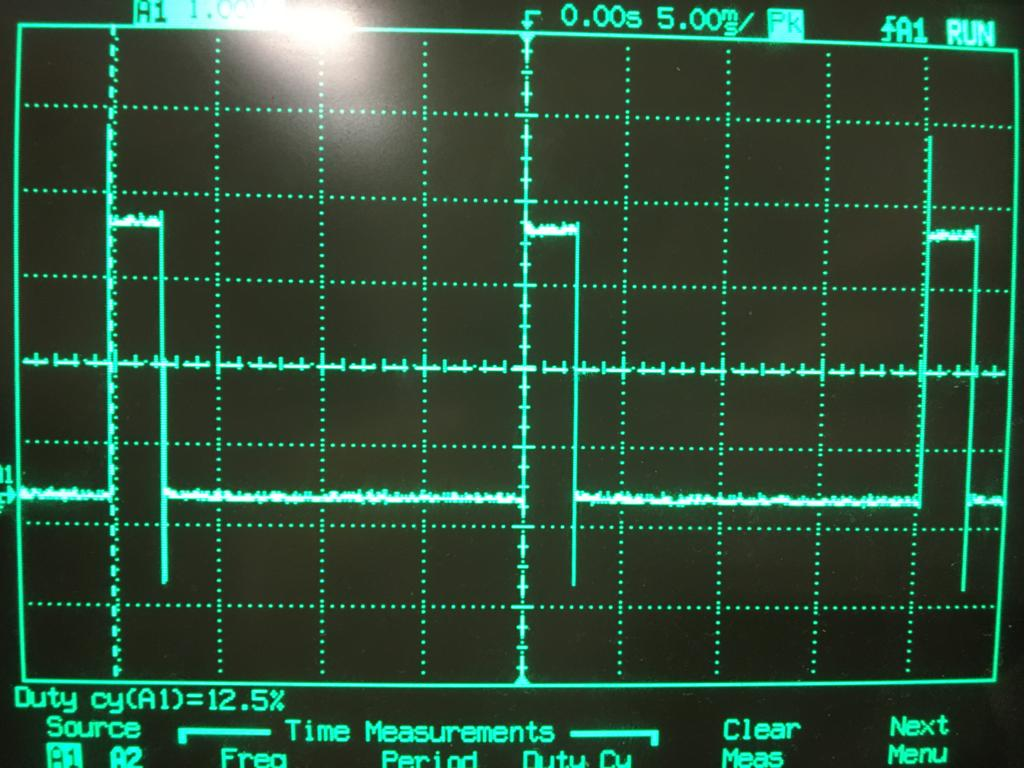
\includegraphics[width=\linewidth]{img/pwm125.jpeg}
     \caption {PWM Signal Duty Cycle = 12.5}
     \label{fig:pwm125}
     \end{subfigure}        
     \caption{Generated PWM signals from the Raspberry Pi}
     \label{fig:pwmaaa}
\end{figure}

\item Generated PWM signals are disturbed while camera is working. Jittering and motor noise occurs. 

\item Obtained images from webcam and raspberry pi camera module can be seen in Figure~\ref{fig:camimages}.

\begin{figure}[ht]
     \centering
     \begin{subfigure}[b]{0.49\textwidth}
     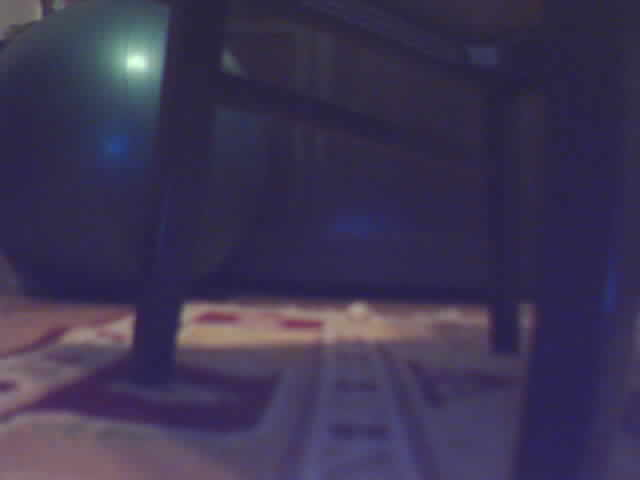
\includegraphics[width=\linewidth]{img/WebCamRPi.jpg}
     \caption{Webcam}
     \label{fig:webcam}
     \end{subfigure}
     \begin{subfigure}[b]{0.49\textwidth}
     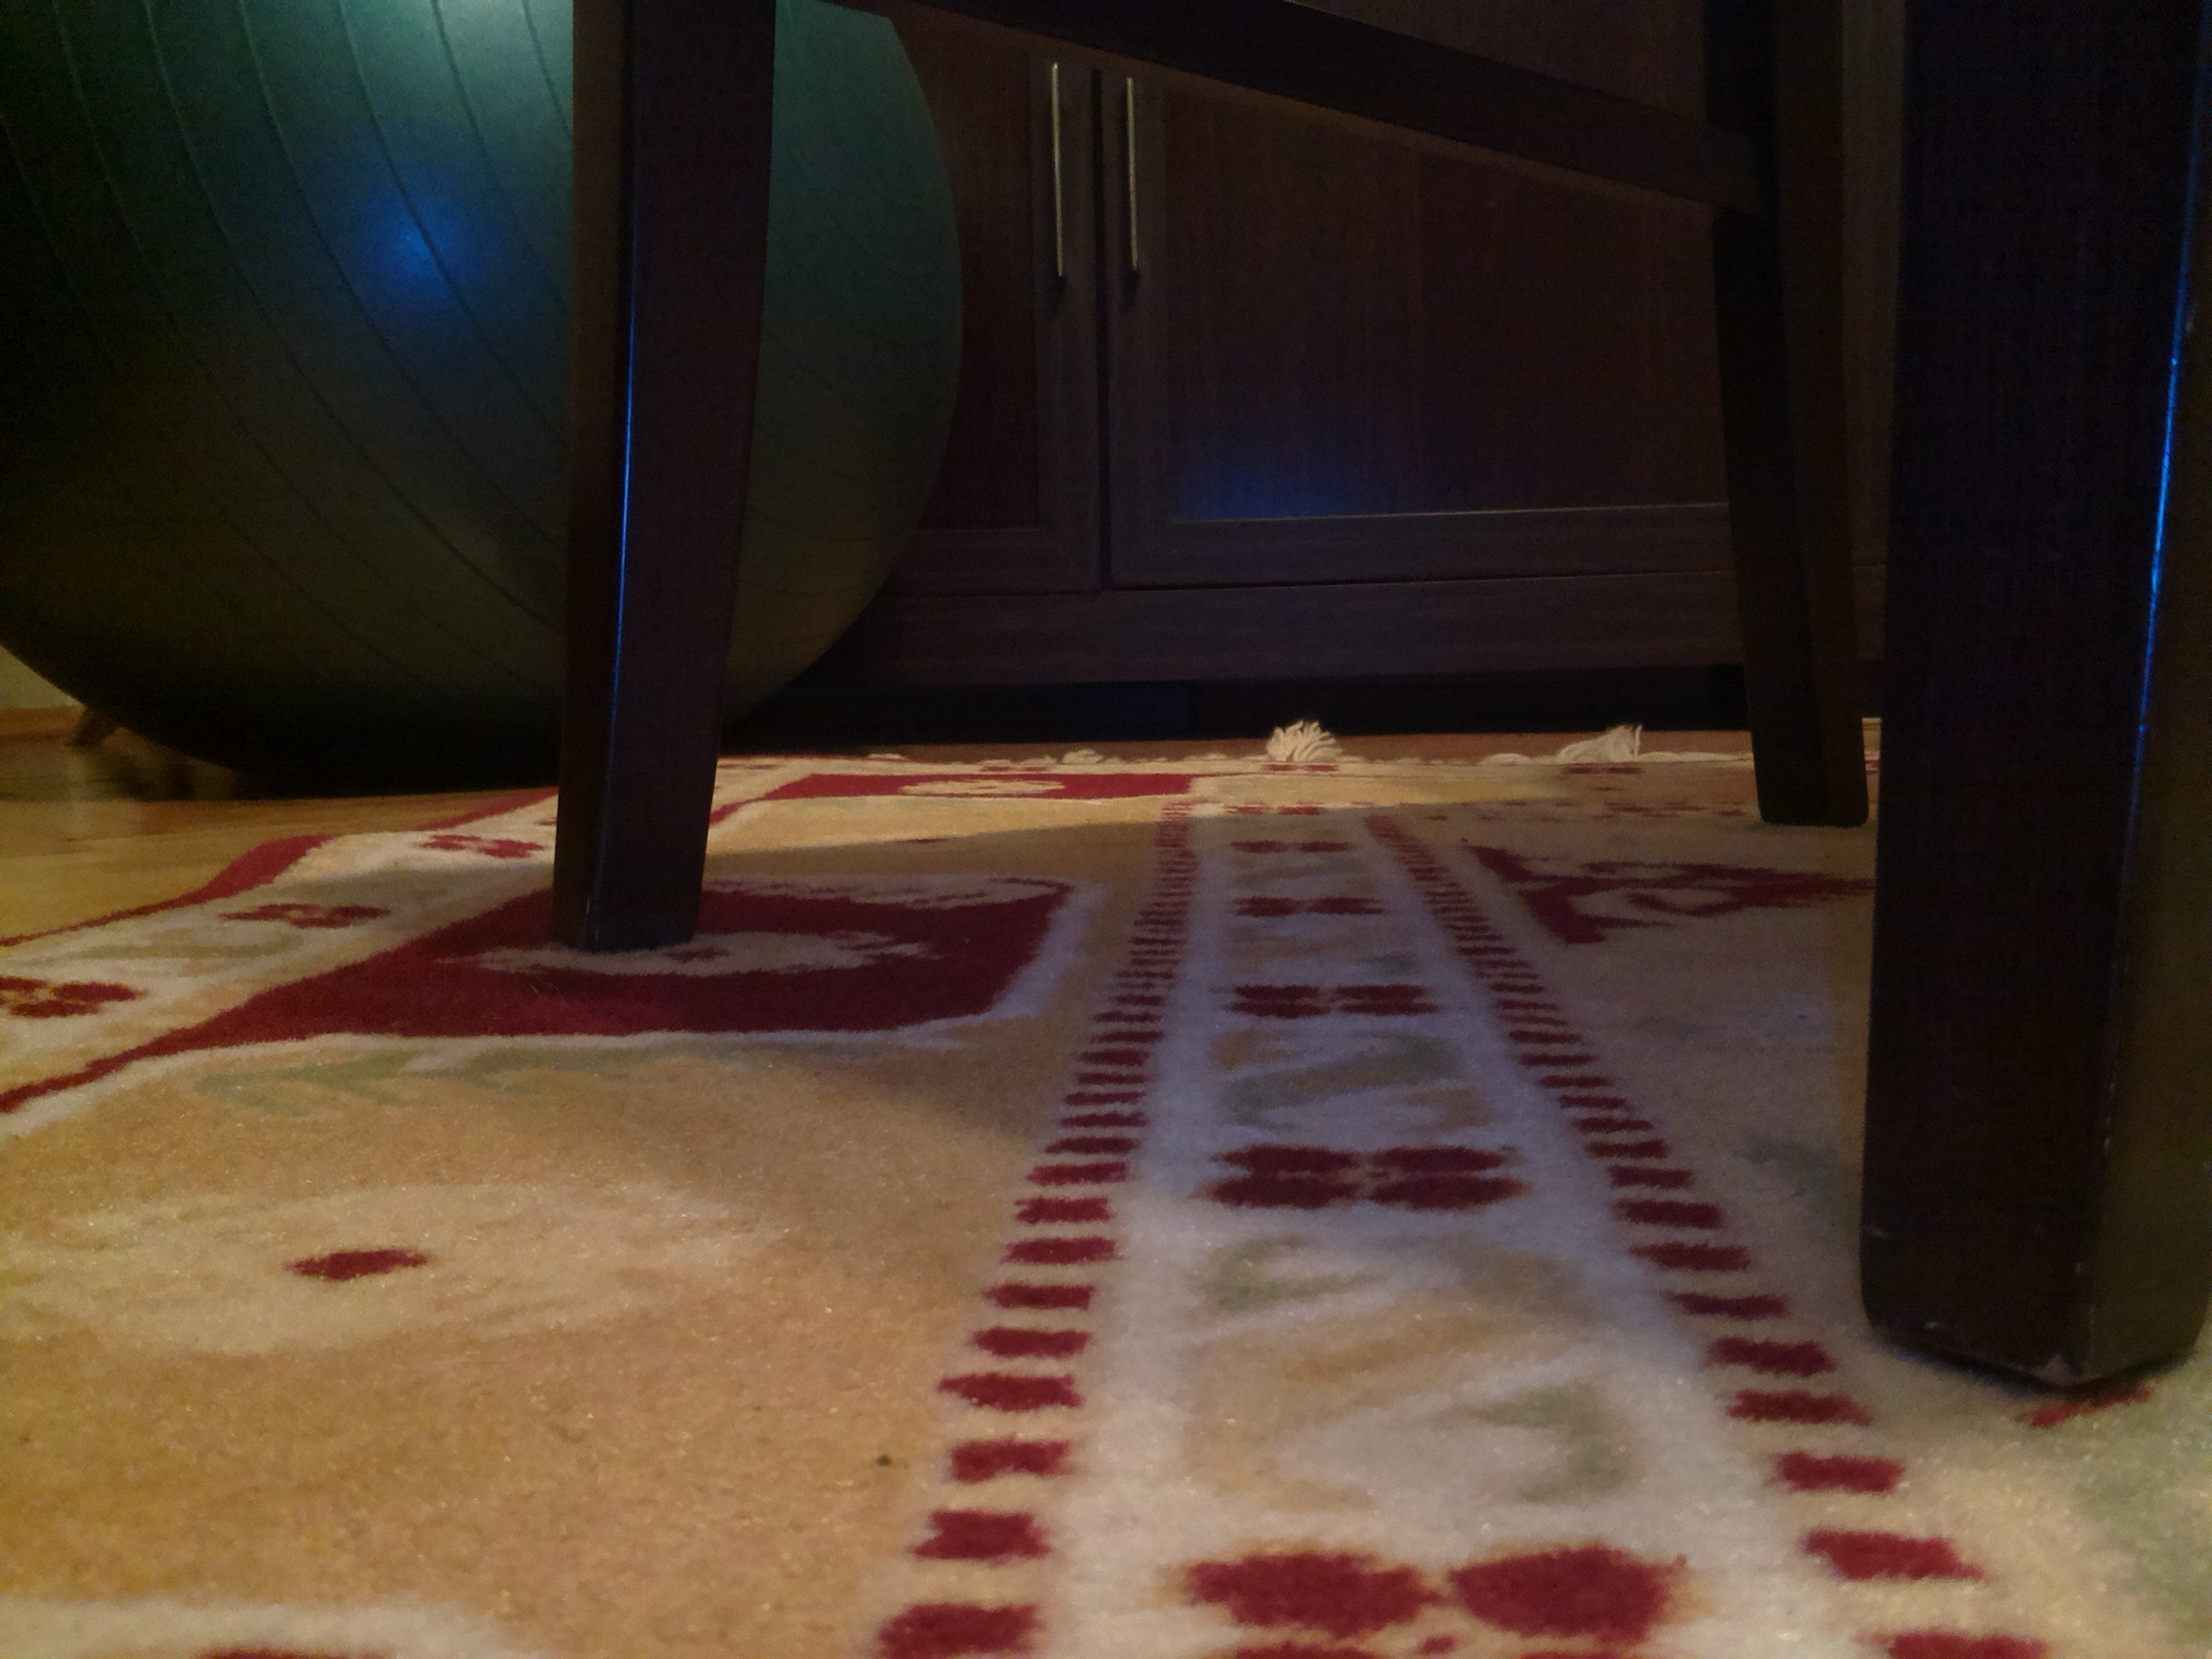
\includegraphics[width=\linewidth]{img/PiCamera.jpg}
     \caption {Raspberry Pi Camera}
     \label{fig:picam}
     \end{subfigure}
     \caption{Comparison of Images Taken on Raspberry Pi Zero}
     \label{fig:camimages}
\end{figure}

\item A dog can be detected from the taken image from the camera with a distance range of 10 cm to 180 cm away from the box. Average detection distance is 110cm. 
\item A cat can be detected from the taken image from the camera with a distance range of 15 cm to 153 cm away from the box.
\item The system draws 0.8 A during the charging operation after the batteries are connected for 4 hours.


%% =========== FATIH - TODO =========== %%

% \item \textcolor{red} { Kamera calısırkenki akım lazım}

%% =========== FATIH - TODO =========== %%

\end{itemize}

% ===== Justification of requirements ===== %
  \subsubsection{Evaluation of Test Results}
\begin{itemize}
\item Batteries are able to operate more than 5 hours. Also, system operates properly with power bank. Since Li-Ion batteries are cheaper, in the design of system Li-Ion batteries will be used. Li-Po batteries will not be tested since first solution operates as required. The subsystem requirement for the battery duration is satisfied.
\item Parallel charging operates as required. The subsystem requirement for re-chargeability is satisfied.
%düzeldi la niye degistiriyon lan neydi sdkjfhsdkjfhs geri al asdjsad
\item Batteries are placed in a small case that is screwed into the box. The subsystem requirement for non-removable batteries is satisfied.
\item 5 V regulator outputs voltages between 5.35 V and 5.45 V for the battery input voltage levels. This is undesired, however does not cause any faults for the raspberry pi.
\item Solders and connectors are used in wiring. The subsystem requirement for proper wiring is satisfied.
\item The raspberry pi operates with the battery connections. The subsystem requirement for operating the raspberry pi is satisfied.
\item The subsystem operates properly during charging. The subsystem requirement is satisfied.
\item The images are obtained successfully from the webcam and raspberry pi camera. The output images can be seen in Figure~\ref{fig:camimages}. When the images taken from the same position are compared, the quality of the image taken with the webcam is very low. Raspberry pi camera module, though more expensive than the webcam, will be used in the final design, since the image quality is vital for every module of the 'Computer Vision' subsystem.
\item The cat should be 15 cm away from the camera in order to obtain successful classification results.
\item The maximum distance between the cat and camera for an accurate classification is 153 cm. This distance is a positive result, the foods will be served before the cat arrives at the box.

\item Noise generated by the camera module propagates through the system finally affecting PWM generation and motor drive. Possible solutions are listed in the anticipated difficulties subsection of electronics subsection.
%There are two possible solutions which are to stand by the camera for a while when feeding the cat and using external motor driver. Algorithm update are going to be tested, followed by motor driver solutions only in case of failure of algorithmic solutions. %UTKU -bunu anticipated difficulties kısmına ekliyorum
% TODO - FATIH bu kotu bir sey dikkatini cekiyorum buraya -- OLMUS MU?
 
\item The drawn currents are low, but the overall system current is not measured. The subsystem requirement for minimum power consumption is partially satisfied.
\item The total charging time will be around 12 hours, which can be considered a long time. However, the system will be able to operate for much more than 5 hours. The subsystem requirement for charging time is not satisfied, but the charging time can be decreased by using lower capacity batteries.

\item The distance between the top of the reservoir and the food level can be measured from the ultrasonic sonar sensor. However, when this distance is shorter than 2 cm, it returns false output. This problem can be solved easily by putting the sensor 2.5 cm above the maximum level of reservoir and rescaling the code in order to obtain correct volume percentage. Since ultrasonic sonar sensor operates properly, infrared sensor will not be tested.
% \item The overall electronics subsystem operates properly except the motor noise problem, which happens when the subsystem is integrated with the mechanical and computer vision parts.

%% TODO - FATIH bu son cumle buyuk bir sikinti gibi - direk cikaralim bunu cok manali degil bence

% ok sure

\end{itemize}

% ===== Comparison with alternative solutions ===== %



% ===== Error sources, their impact and ways to mitigate ===== %


\subsection{Plans}

\begin{itemize}
\item Fuses will be added in order to obtain a safe system.
\item Motor noise will be eliminated/minimized.
\item Weight sensor will be tested and integrated to the subsystem.
\item Analog voltage level of the batteries will be taken from one of the GPIO pins of the raspberry pi and percentage value will be observable in the web interface.
\item Voltage level indicator will be added to the box. 
%% TODO - FATIH emin konussak daha iyi olur ??
\item Dog deterring system will be integrated to the subsystem.
\end{itemize}

% ===== State names of responsible person/people ===== %


\subsection{Anticipated Difficulties}
%There are two possible solutions which are to stand by the camera for a while when feeding the cat and using external motor driver. Algorithm update are going to be tested, followed by motor driver solutions only in case of failure of algorithmic solutions.
\begin{enumerate}
\item PWM signal is disturbed while the camera is working. Possible solutions are listed below.
\begin{itemize}
\item Using capacitors at the input of servo motor and output of batteries. By this way, motor noise can be suppressed since the noise will be filtered. \cite{cite:polulu}

\item Using ferrite choke in order to eliminate high frequency noise. \cite{cite:analog}
\item Applying more complex high pass filters.
\item Using twisted cables  to reduce the magnetic field noise. \cite{cite:robotshop}
\item Using motor drivers.
\end{itemize}
These solutions will be tested in the listed order until a satisfactory result is achieved.
\item Adjustable regulator heats up while driving the servo motor. Possible solutions are listed below.
\begin{itemize}
\item Using a regulator with a better cooling system.
\item Directly connecting separate batteries to the power inputs of the motor, with the help of relays.
\end{itemize}

\end{enumerate}

\subsection{Test Plans}
\begin{itemize}
\item PWM signal will be tested while all other subsystems are working step by step applying the solution methods listed in the anticipated difficulties section of the electronics subsystem.
\item New regulator connected to the servo motor will be tested.
\item Weight sensor will be tested.
\item Voltage level indicator will be tested.
\item Dog deterring system will be tested.
\item Overall system power consumption will be measured.
\item Overall system will be tested after the fuses are added.
\end{itemize}

\subsubsection{Test Procedure}
\begin{itemize}
\item Test the battery duration after all of them are fully charged while all subsystems are operating.
\item Test the motor for 200 rotation cycles to see how well it behaves. %%ben bakarim
\item Test the voltage level indicator during charging and non charging periods.
\item Test the volume level indicator with the motor rotation.
\end{itemize}


% ===== Measure of success ===== %

